\chapter{Design and Analysis of the Dental Surgical Robot - DentiBot}
\label{chapter3}
\section{Requirement and Specification}
\label{sec:requirement}
\hspace*{6mm}The dental surgical robot should enable dentists to perform delicate and complicated surgery operations because the average diameter of a root canal is $0.28 (\pm 0.08)$ mm \cite{wu2002does}. Therefore, our system should have a high resolution of movement. Next, an appropriate workspace is required. In dental anatomy, teeth are located on the maxillary (lower jaw) and the mandibular (upper jaw). To perform surgery with both sides, we should rotate the end effector at least $180$ degrees. Also, there is a previous research, which shows the average range of maximum mouth opening is 50.3 mm ± 6.26 mm \cite{agrawal2015evaluation}. Hence, the end effector of our system should be less than this range.
\section{Design of the DentiBot}
\hspace*{6mm}As discussed in the previous section, we decide to build a system composed of a robot arm, an F/T sensor, and a modified handpiece. Why we choose a robot arm and an F/T sensor is because we want to mimic the dentist's motion. Due to the 6-DOF robot arm, we can achieve the action with less hardware restriction. We can easily move to almost desired positions and rotate more than 180 degrees to drill tooth in both sides of mouth. Also, with the 6-DoF F/T sensor, we can take the real-time force and torque feedbacks as haptic feedback. Our system can take reaction with the F/T sensor such as a dentist touch something in the surgery and do the corresponding reaction. Besides, by modifying the existing handpiece, which is a handheld dental electric device, we do not worry about the workspace and dimension in the mouth.		
\par
\begin{figure}[H]
\begin{center}
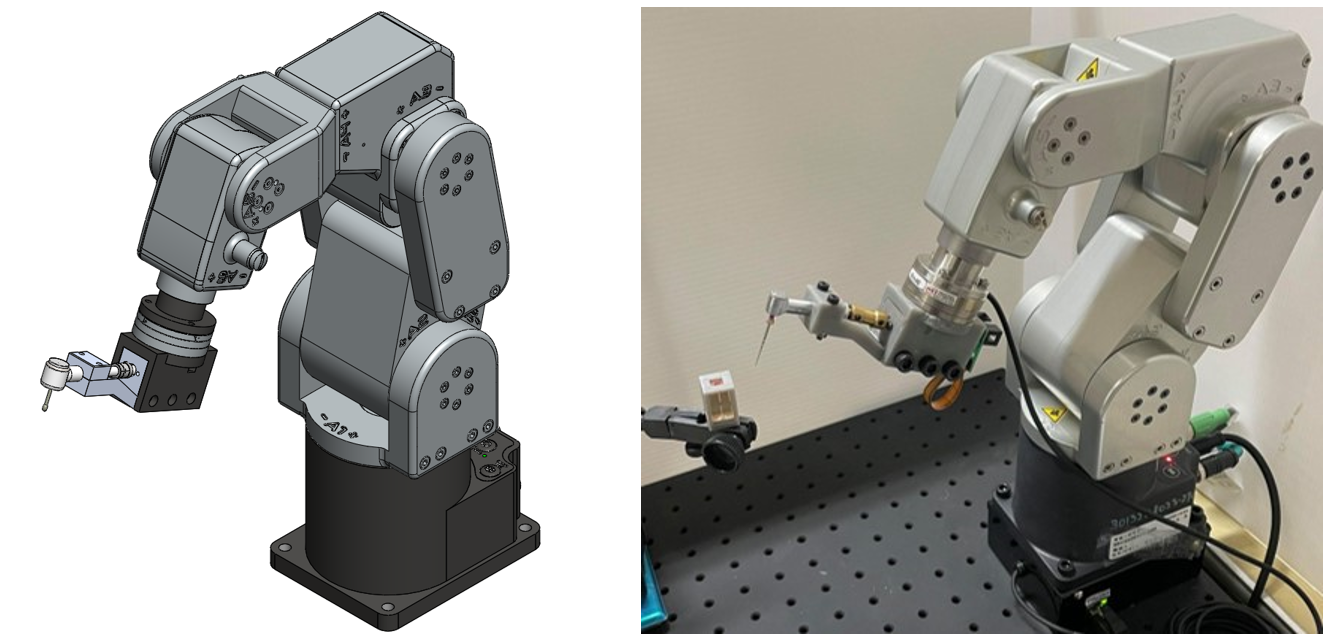
\includegraphics[width=1\linewidth]{Images/DentiBot.png}
\caption{
The DentiBot and an acyclic tooth model
}\label{fig:DentiBot}
\end{center}
\end{figure}	
To meet the requirement of workspace and dimension, we have to select suitable devices according to those requirements as shown in Fig \ref{fig:DentiBot}. First, We choose Meca500 manufactured by Mecadamic Inc. as our 6-DOF robot arm  \cite{web4} . Its feature is high repeatability (precision: 5 \textmu m), and it is equipped with zero-backlash speed reducers. In addition, it is compact and portable for laboratory investigation. Second, Mini40 manufactured by ATI Inc. is the corresponding F/T sensor with three force and three torque detections \cite{web5}. As for the end effector, we modify an existing dental handpiece that equips a file exchange mechanism shown in Fig \ref{fig:modified_handpiece}. The rotation of endodontic file   is driven by a servo motor. The modified handpiece with a motor total weighs around 139 grams.  Also, Adapters are designed to assemble these devices.
\par
\begin{figure}[htbp]
\begin{center}
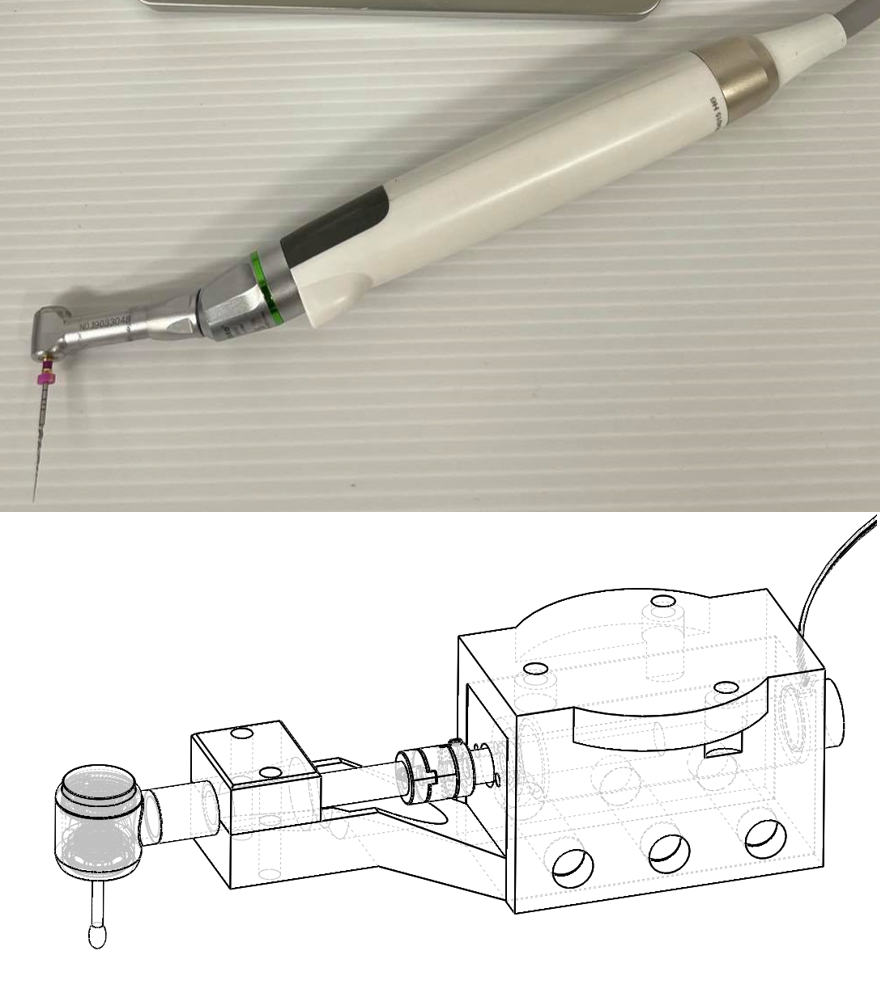
\includegraphics[width=0.7\linewidth]{Images/modified_handpiece.png}
\caption{
Modified handpiece
}\label{fig:modified_handpiece}
\end{center}
\end{figure}	
Therefore, DentiBot totally has seven degrees of freedom. Six degree of freedom come from Meca500, and the other thanks to our modified handpiece. The rotation of the root canal file is driven by a servo motor whose maximum rotation speed is more than 600 rpm.
																
\section{Kinematics Analysis}
\label{sec:kinematics}
\hspace*{6mm}The purpose of this section and section \ref{sec:ref_robot} is to serve as a tutorial and provide some crucial approaches when combining a robot arm and an end effector. We derive the forward and inverse kinematics in section \ref{sec:forward} and describe the Jacobian matrix in section \ref{sec:jacobian}. 
\subsection{Coordinate Definition}
\hspace*{6mm}In Fig \ref{fig:frames} , we define frame\{0\} to frame\{6\} which represent each frame of axes of the Meca500, frame\{S\} which represent the frame of the ATI-mini40 and frame\{H\} which represent the frame of the handpiece.
\begin{figure}[htbp]
\begin{center}
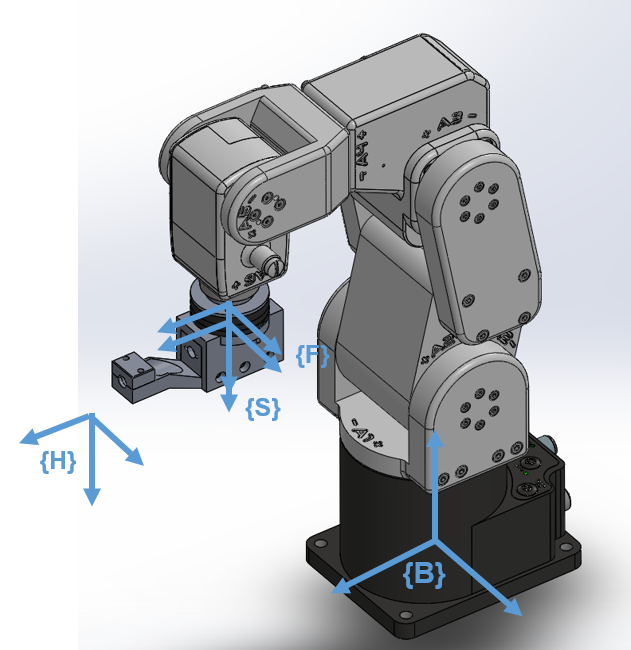
\includegraphics[width=0.72\linewidth]{Images/Coordinates.png}
\caption{
Coordinate Definition
}\label{fig:frames}
\end{center}
\end{figure} 
\subsection{Forward and Inverse Kinematics}
\label{sec:forward}
\begin{table}[htbp]
\centering
\caption{Denavit-Hartenberg parameters of Meca500}
\label{tab:DHtable}
\begin{tabular}{ccccc} 
\hline \hline
$i$ (link number)		&$\alpha _{i-1}$ (deg)	&$a_{i-1}$ (mm)	& $\theta _i$ (deg)			&$d_i$ (mm)	\\
\hline
1   					&0    					&0				&$\theta _1$				&135 \\
2   					&-90   					&0				&$\theta _2-90$				&0 \\
3  						&0    					&135			&$\theta _3$ 				&0 \\
4   					&-90    				&38				&$\theta _4$ 				&120 \\
5   					&90   					&0				&$\theta _5$ 				&0 \\
6						&-90  					&0				&$\theta _6+180$ 				&70 \\
\hline\hline
\end{tabular}
\end{table}
\hspace*{6mm}Denavit-Hartenberg parameters are shown as Table \ref{tab:DHtable}. Then, the forward kinematics of Meca500 is derived as
\begin{equation}
\begin{split}
^0_6\mathbf{T} =
\ ^0_1\mathbf{T} \cdot \ ^1_2\mathbf{T} \cdot \ ^2_3\mathbf{T} \cdot \ ^3_4\mathbf{T} \cdot \ ^4_5\mathbf{T} \cdot \ ^5_6\mathbf{T} =
\begin{bmatrix}
^0_6\mathbf{R}	&^0\boldsymbol{p}_\mathrm{6org}\\
0				&1\\
\end{bmatrix}\\
\end{split}
\end{equation}\label{eq:translation matrix}
where $^0_6\mathbf{R}$ is the rotation matrix from frame\{6\} to frame\{0\}, $^0\boldsymbol{p}_\mathrm{6org}$ is the origin of the frame\{6\} observed from frame\{0\}. All detailed indexes of $^0_6\mathbf{T}$ are shown as Appendix \ref{appendix:forward}
\par
Incidentally, there is an alternative to calculate the transformation matrix of Meca500. We can use command "GetPose" to obtain (x,y,z,$\alpha$,$\beta$,$\gamma$). Then, we can use this information to derive the following equation.
\begin{equation}
\begin{split}
^0_6\mathbf{T} 
&= 
\begin{bmatrix}
\mathbf{R_x(\alpha ) \cdot R_y(\beta ) \cdot R_z(\gamma )} 
& \begin{matrix}
x\\ 
y\\ 
z
\end{matrix}\\ 
0 & 1
\end{bmatrix}\\
&= 
\begin{bmatrix} 
c_\beta c_\gamma 										& -c_\beta s_\gamma 									& s_\beta 					&x\\ 
c_\alpha s_\gamma +  s_\alpha s_\beta c_\gamma 			& c_\alpha c_\gamma -  s_\alpha s_\beta s_\gamma		& -s_\alpha c_\beta			&y\\ 
s_\alpha s_\gamma -  c_\alpha s_\beta c_\gamma 			& s_\alpha c_\gamma +  c_\alpha s_\beta s_\gamma 		& c_\alpha c_\beta 			&z\\ 
0 														&0 														&0							&1
\end{bmatrix}
\end{split}
\end{equation}
where $C_{\star} $, $ S_{\star}$ denote $\cos \left(\star \right)$, $\sin \left(\star \right)$; $\alpha ,\beta ,\gamma$ are in representation of Euler angle.
\subsection{Jacobian matrix} 
\label{sec:jacobian}
\hspace*{6mm}Here we evaluate geometric Jacobian based on frame\{0\}, geometric Jacobian based on frame\{6\} and analytical Jacobian.
\par
First and foremost, we should clarify the difference between geometric Jacobian and analytical Jacobian. They both use the same linear velocity but consider different angular velocity. The angular velocity which geometric Jacobian applies is relevant to the axis angles ($\theta _x$,$\theta _y$,$\theta _z$). In contrast, the angular velocity which analytical Jacobian contemplates is related to the orientation ($\alpha$,$\beta$,$\gamma$) of the end effector.
\subsubsection{Geometric Jacobian Based on Frame\{0\}}
Before examining the geometric Jacobian matrix, it will be necessary to find the relationship between the position and joints' angles and the relationship between the axis angle and the joints' angles.
\par\noindent
Based on the translation matrix in Equation \ref{eq:translation matrix}, we obtain the relationship between the position and joints' angles.
\begin{equation}
\label{eq:lin vel}
\begin{split}
^0\boldsymbol{p}_\mathrm{6org}
= 
\begin{bmatrix}
x\\
y\\
z\\
\end{bmatrix} 
=
\begin{bmatrix}
x(\theta _1, \theta _2, \cdots, \theta _6)\\
y(\theta _1, \theta _2, \cdots, \theta _6)\\
z(\theta _1, \theta _2, \cdots, \theta _6)
\end{bmatrix} 
\end{split}
\end{equation}
Moreover, we dissect the relationship between the axis angle and joints' angles.
\begin{equation}
\label{eq:ang vel_axis}
\begin{split}
\begin{bmatrix}
\theta _x \\
\theta _y \\
\theta _z 
\end{bmatrix}
=
\ ^0_1\mathbf{R}
\begin{bmatrix}
0 \\ 
0 \\ 
\theta _1
\end{bmatrix}
+
\ ^0_2\mathbf{R}
\begin{bmatrix}
0 \\ 
0 \\ 
\theta _2
\end{bmatrix}
+
\ ^0_3\mathbf{R}
\begin{bmatrix}
0 \\ 
0 \\ 
\theta _3
\end{bmatrix}
+
\ ^0_4\mathbf{R}
\begin{bmatrix}
0 \\ 
0 \\ 
\theta _4
\end{bmatrix}
+
\ ^0_5\mathbf{R}
\begin{bmatrix}
0 \\ 
0 \\ 
\theta _5
\end{bmatrix}
+
\ ^0_6\mathbf{R}
\begin{bmatrix}
0 \\ 
0 \\ 
\theta _6
\end{bmatrix}
\end{split}
\end{equation}
We can differentiate Equation \ref{eq:lin vel} and \ref{eq:ang vel_axis} to obtain Jacobian matrices.
\begin{equation}
\begin{split}
\boldsymbol{v} 
= 
\begin{bmatrix}
\dot{x}\\
\dot{y}\\
\dot{z}
\end{bmatrix}
=
\mathbf{J_{gv}} \cdot \boldsymbol{\dot{q}}
,\ 
\boldsymbol{w} 
= 
\begin{bmatrix}
\dot{\theta _x}\\
\dot{\theta _y}\\
\dot{\theta _z}
\end{bmatrix}
=
\mathbf{J_{gw}} \cdot \boldsymbol{\dot{q}}
\end{split}
\end{equation}
where
\begin{equation*}
\begin{split}
\mathbf{J_{gv}} =
\begin{bmatrix}
\frac{\partial x}{\partial \theta _1}	&\frac{\partial x}{\partial \theta _2}	&\cdots		&\frac{\partial x}{\partial \theta _6}\\
\frac{\partial y}{\partial \theta _1}	&\frac{\partial y}{\partial \theta _2}	&\cdots		&\frac{\partial y}{\partial \theta _6}\\
\frac{\partial z}{\partial \theta _1}	&\frac{\partial z}{\partial \theta _2}	&\cdots		&\frac{\partial z}{\partial \theta _6}
\end{bmatrix}
,\ \mathbf{J_{gw}} = 
\begin{bmatrix}
\frac{\partial \theta _x}{\partial \theta _1}	&\frac{\partial \theta _x}{\partial \theta _2}	&\cdots		&\frac{\partial \theta _x}{\partial \theta _6}\\
\frac{\partial \theta _y}{\partial \theta _1}	&\frac{\partial \theta _y}{\partial \theta _2}	&\cdots		&\frac{\partial \theta _y}{\partial \theta _6}\\
\frac{\partial \theta _z}{\partial \theta _1}	&\frac{\partial \theta _z}{\partial \theta _2}	&\cdots		&\frac{\partial \theta _z}{\partial \theta _6}
\end{bmatrix} 
,\ \boldsymbol{\dot{q}}
=
\begin{bmatrix}
\dot{\theta _1} \\ 
\dot{\theta _2} \\ 
\dot{\theta _3} \\ 
\dot{\theta _4} \\ 
\dot{\theta _5} \\ 
\dot{\theta _6} 
\end{bmatrix}\\
\end{split}
\end{equation*}
As a result, the geometric Jacobian matrix based on frame{0} $\mathbf{^0J_g}$ is derived as
\begin{equation}
\label{eq:jg0}
\begin{split}
\boldsymbol{\dot{x}} = \ \mathbf{^0\!J_g} \cdot \boldsymbol{\dot{q}}
,\ \ 
\boldsymbol{\dot{q}} = \ \mathbf{^0\!J_g^{-1}} \cdot \boldsymbol{\dot{x}}
\end{split}
\end{equation}
where
\begin{equation}
\begin{split}
\boldsymbol{\dot{x}}
=
\begin{bmatrix}
\dot{x}\\
\dot{y}\\
\dot{z}\\
\dot{\theta _x}\\
\dot{\theta _y}\\
\dot{\theta _z}
\end{bmatrix}_{\!\{0\}}
,\ 
\boldsymbol{\dot{q}}
=
\begin{bmatrix}
\dot{\theta _1} \\ 
\dot{\theta _2} \\ 
\dot{\theta _3} \\ 
\dot{\theta _4} \\ 
\dot{\theta _5} \\ 
\dot{\theta _6} 
\end{bmatrix}
\end{split}
\end{equation}
There is a further derivation. In terms of the Jacobian matrix, we can derive the other property.
\begin{equation}
\begin{split}
\boldsymbol{\tau } = \mathbf{^0\!J^\top _g} \cdot \boldsymbol{f}\ \ \ \ 
\Leftrightarrow \ \ \ \ 
\begin{bmatrix}
\tau_{\theta _1} \\ 
\tau_{\theta _2} \\ 
\tau_{\theta _3} \\ 
\tau_{\theta _4} \\ 
\tau_{\theta _5} \\ 
\tau_{\theta _6} \\ 
\end{bmatrix}
=
\mathbf{^0\!J^\top _g} 
\cdot
\begin{bmatrix}
f_x \\ 
f_y \\ 
f_z \\ 
\tau_{x} \\ 
\tau_{y} \\ 
\tau_{z}
\end{bmatrix}
\end{split}
\end{equation}
where $\boldsymbol{\tau }$ is the vector of joints' torques and $\boldsymbol{f}$ is the vector composed of inertial forces and torques of the robot arm.
\subsubsection{Geometric Jacobian Based on Frame\{6\}}
\label{sec:jg6}
\hspace*{6mm}Why we need geometric Jacobian based on frame\{6\} is that in section \ref{sec:adm ctrl} we will apply admittance control and it will use F/T sensor mounted on frame\{6\} instead of frame\{0\} to detect forces and torques. To start with Equation \ref{eq:jg0}
\begin{equation}
\begin{split}
\begin{bmatrix}
\dot{x}\\
\dot{y}\\
\dot{z}\\
\dot{\theta _x}\\
\dot{\theta _y}\\
\dot{\theta _z}
\end{bmatrix}_{\!\{0\}}
=
\mathbf{^0\!J_g} \cdot 
\begin{bmatrix}
\dot{\theta _1} \\ 
\dot{\theta _2} \\ 
\dot{\theta _3} \\ 
\dot{\theta _4} \\ 
\dot{\theta _5} \\ 
\dot{\theta _6} 
\end{bmatrix}\\
\end{split}
\end{equation}
Then, left-multiply a matrix. 
\begin{equation}
\label{eq:jg6_leftmul}
\begin{split}
\begin{bmatrix}
^0_6\mathbf{R} & 0_{ 3\times 3} \\ 
0_{ 3\times 3} & ^0_6\mathbf{R}
\end{bmatrix}
\begin{bmatrix}
\dot{x}\\
\dot{y}\\
\dot{z}\\
\dot{\theta _x}\\
\dot{\theta _y}\\
\dot{\theta _z}
\end{bmatrix}_{\!\{0\}}
=
\begin{bmatrix}
^0_6\mathbf{R} & 0_{ 3\times 3} \\ 
0_{ 3\times 3} & ^0_6\mathbf{R}
\end{bmatrix}
\mathbf{^0\!J_g} \cdot 
\begin{bmatrix}
\dot{\theta _1} \\ 
\dot{\theta _2} \\ 
\dot{\theta _3} \\ 
\dot{\theta _4} \\ 
\dot{\theta _5} \\ 
\dot{\theta _6} 
\end{bmatrix}\\
\end{split}
\end{equation}
According to the transformation coordinate relationship between frame\{0\} and frame\{6\},
\begin{equation}
\begin{split}
\begin{bmatrix}
\dot{x}\\ 
\dot{y}\\ 
\dot{z}\\ 
\dot{\theta_x}\\ 
\dot{\theta_y}\\
\dot{\theta_z} 
\end{bmatrix}_{\!\{6\}}
=
\begin{bmatrix}
^0_6\mathbf{R} & 0_{ 3\times 3} \\ 
0_{ 3\times 3} & ^0_6\mathbf{R}
\end{bmatrix}
\begin{bmatrix}
\dot{x}\\ 
\dot{y}\\ 
\dot{z}\\ 
\dot{\theta_x}\\ 
\dot{\theta_y}\\
\dot{\theta_z} 
\end{bmatrix}_{\!\{0\}}
\end{split}
\end{equation}
substitute it into Eq \ref{eq:jg6_leftmul}, we can observe an essential equation.
\begin{equation}
\begin{split}
\mathbf{^6\!J_g}
= 
\begin{bmatrix}
^0_6\mathbf{R} & 0_{ 3\times 3} \\ 
0_{ 3\times 3} & ^0_6\mathbf{R}
\end{bmatrix}
\cdot
\mathbf{^0\!J_g}
\end{split}
\end{equation}
Notably,
\begin{equation}
\label{eq:jg6}
\begin{split}
\boldsymbol{\dot{x}} = \ \mathbf{^6\!J_g} \cdot \boldsymbol{\dot{q}}
,\ \ 
\boldsymbol{\dot{q}} = \ \mathbf{^6\!J_g^{-1}} \cdot \boldsymbol{\dot{x}}
\end{split}
\end{equation}
where
\begin{equation*}
\begin{split}
\boldsymbol{\dot{x}}
=
\begin{bmatrix}
\dot{x}\\
\dot{y}\\
\dot{z}\\
\dot{\theta _x}\\
\dot{\theta _y}\\
\dot{\theta _z}
\end{bmatrix}_{\!\{6\}}
,\ 
\boldsymbol{\dot{q}}
=
\begin{bmatrix}
\dot{\theta _1} \\ 
\dot{\theta _2} \\ 
\dot{\theta _3} \\ 
\dot{\theta _4} \\ 
\dot{\theta _5} \\ 
\dot{\theta _6} 
\end{bmatrix}
\end{split}
\end{equation*}
\subsubsection{Analytical Jacobian}
\hspace*{6mm}The linear velocity of analytical Jacobian and geometric Jacobian is the same as shown in Eq \ref{eq:lin vel}. Nevertheless, as for angular velocity, analytical Jacobian takes the orientation ($\alpha$,$\beta$,$\gamma$) of the end effector into consideration. First of all, we investigate the relationship between the axis angle and the orientation of the end effector as following.
\begin{equation}
\begin{split}
\begin{bmatrix}
\theta _x \\ 
\theta _y \\ 
\theta _z
\end{bmatrix}
&=
\begin{bmatrix}
\alpha \\ 
0\\ 
0
\end{bmatrix}
+
R_x(\alpha)
\begin{bmatrix}
0 \\ 
\beta \\ 
0
\end{bmatrix}
+
R_x(\alpha)R_y(\beta)
\begin{bmatrix}
0 \\ 
0\\ 
\gamma
\end{bmatrix}\\
&=
\begin{bmatrix}
1 & 0 & S_\beta \\ 
0 & C_\alpha & -S_\alpha C_\beta \\ 
0 & S_\alpha & C_\alpha C_\beta
\end{bmatrix}
\begin{bmatrix}
\alpha \\ 
\beta\\ 
\gamma
\end{bmatrix}
\end{split}
\end{equation}
Then, utilize this generalized vector to get its Jacobian matrix $\mathbf{J_{we}}$.
\begin{equation}
\begin{split}
\begin{bmatrix}
\dot{\theta _x} \\ 
\dot{\theta _y} \\ 
\dot{\theta _z}
\end{bmatrix}
=
\mathbf{J_{\!we}}
\cdot
\begin{bmatrix}
\dot{\alpha} \\ 
\dot{\beta} \\ 
\dot{\gamma}
\end{bmatrix}
\end{split}
\end{equation}
where
\begin{equation}
\label{eq:jacobian_euler}
\begin{split}
\mathbf{J_{we}}
=
\begin{bmatrix}
1														& \gamma C_{\beta}							& S_{\beta}\\
- \beta S_{\alpha} -  \gamma C_{\alpha}C_{\beta}		& C_{\alpha} +  \gamma S_{\alpha}S_{\beta}	& -C_{\beta}S_{\alpha}\\
\beta C_{\alpha} -  \gamma C_{\beta}S_{\alpha}			& S_{\alpha} -  \gamma C_{\alpha}S_{\beta}	&  C_{\alpha}C_{\beta}
\end{bmatrix}
\end{split}
\end{equation}
Therefore,
\begin{equation}
\begin{split}
\begin{bmatrix}
\dot{x} \\
\dot{y} \\
\dot{z} \\
\dot{\theta _x} \\
\dot{\theta _y} \\
\dot{\theta _z} 
\end{bmatrix}
=
\begin{bmatrix}
\mathbf{I}_{3\times 3} & 0_{3\times 3}\\
0_{3\times 3} & \mathbf{J_{we}}
\end{bmatrix}
\begin{bmatrix}
\dot{x} \\
\dot{y} \\
\dot{z} \\
\dot{\alpha} \\ 
\dot{\beta} \\ 
\dot{\gamma} 
\end{bmatrix}
\end{split}
\end{equation}
Finally, we obtain the relationship between geometric and analytical Jacobian.
\begin{equation}
\begin{split}
\mathbf{J_g} = 
\begin{bmatrix}
\mathbf{I}_{3\times 3} & 0_{3\times 3}\\
0_{3\times 3} & \mathbf{J_{we}}
\end{bmatrix}
\mathbf{J_a},\ 
\mathbf{J_g} = 
\begin{bmatrix}
\mathbf{I}_{3\times 3} & 0_{3\times 3}\\
0_{3\times 3} & \mathbf{J_{we}^{-1}}
\end{bmatrix}
\mathbf{J_a}
\end{split}
\end{equation}

\section{Coordinate Transformation of the Robot Arm}
\label{sec:ref_robot}
\hspace*{6mm}So far, with the forward and inverse kinematics, the robot arm can translate and rotate around frame\{6\}. However, we do not see the origin of the frame\{6\} as an operating point. Because the F/T sensor and a detachable end effector will be both mounted on the wrist, the tooltip position is what we want. That means we should let the robot arm know how to translate and rotate in frame\{T\} instead of frame\{6\}. If we have translation and rotation information of the tooltip, there is an easy way to directly give the above information to the robot arm. SetTRF (x,y,z,$\alpha$,$\beta$,$\gamma$) is the command of the robot arm, whose (x,y,z) is translation vector and ($\alpha$,$\beta$,$\gamma$) is rotation vector in representation of Euler angle .
\par
To obtain translation and rotation vector, we respectively introduce Tool Center Point in section \ref{sec:tcp} to find the translation vector and propose an approach in section \ref{sec:rot inf} to find the rotation vector.							
\subsection{Translation Analysis - Tool Center Point}
\label{sec:tcp}
\begin{figure}[htbp]
\begin{center}
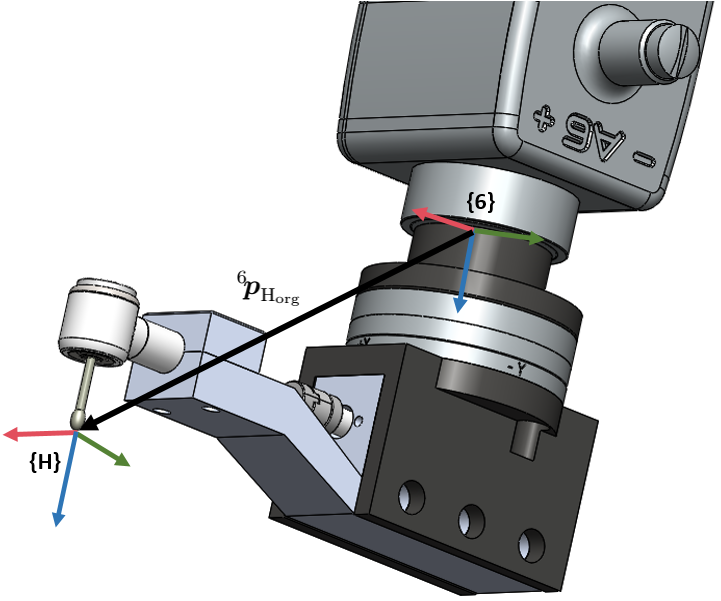
\includegraphics[width=0.7\linewidth]{Images/TCP.png}
\caption{
Schematic diagram for Tool Center Point. The translation vector $^\mathrm{6}\!\boldsymbol{p}_\mathrm{H_{org}}$ denotes the origin position relative to the frame\{6\}.
}\label{fig:tcp}
\end{center}
\end{figure}
\hspace*{6mm}Tool Center Point (TCP) is a critical problem for robot arm control \cite{yang2017four}. In the previous section, we have calculated the forward and inverse kinematics of the robot arm. By Calculating kinematics, we can keep track of the origin of the frame\{6\}, which is observed from the base frame. The robot arm has the capability to translate and rotate with the origin of the frame\{6\}. The overhead motions are like a remote center motion (RCM). We should find the position of the tooltip and make it be an RCM point. Nevertheless, it's inefficient to recalculate the transformation matrix via mechanism dimension when changing an end effector or a tool (root canal reamer).
\par
In order to overcome this problem, we interpret the four-points method to obtain the tooltip position, which is also the translation vector.
\par\noindent
From Fig \ref{fig:frames}, we can obtain the following transformation matrix,
\begin{equation}
\begin{split}
_{\mathrm{H}}^{\mathrm{B}}\mathbf{T} &=\ _{\mathrm{6}}^{\mathrm{B}}\mathbf{T}\cdot \ _{\mathrm{H}}^{\mathrm{6}}\mathbf{T}\\
\end{split}
\end{equation}		
and it can be rewritten as
\begin{equation}
\begin{split}																												
\begin{bmatrix}
_{\mathrm{H}}^{\mathrm{B}}\mathbf{R} & ^\mathrm{B}\!\boldsymbol{p}_\mathrm{H_{org}}\\ 
0 & 1
\end{bmatrix} &=
\begin{bmatrix}
_{\mathrm{6}}^{\mathrm{B}}\mathbf{R} & ^\mathrm{B}\!\boldsymbol{p}_\mathrm{6_{org}}\\ 
0 & 1
\end{bmatrix}
\begin{bmatrix}
_{\mathrm{H}}^{\mathrm{6}}\mathbf{R} & ^\mathrm{6}\!\boldsymbol{p}_\mathrm{H_{org}}\\ 
0 & 1
\end{bmatrix}\\
%----------------------------------------------------------------------------------------------------------------------------
&= 
\begin{bmatrix}
_{\mathrm{6}}^{\mathrm{B}}\mathbf{R} \cdot _{\mathrm{H}}^{\mathrm{6}}\!\mathbf{R} & _{\mathrm{6}}^{\mathrm{B}}\mathbf{R} \cdot ^\mathrm{6}\!\!\boldsymbol{p}_\mathrm{H_{org}} +\ ^\mathrm{B}\!\boldsymbol{p}_\mathrm{6_{org}}\\ 
0 & 1
\end{bmatrix}\\
\end{split}
\end{equation}
Consequently, we get a crucial equation:
\begin{equation}
\begin{split}
^\mathrm{B}\!\boldsymbol{p}_\mathrm{H_{org}} &=\  _{\mathrm{6}}^{\mathrm{B}}\mathbf{R}\cdot\ ^\mathrm{6}\!\boldsymbol{p}_\mathrm{H_{org}} +\ ^\mathrm{B}\!\boldsymbol{p}_\mathrm{6_{org}}\\
\end{split}
\end{equation}
Now, we move the tooltip to a fixed point with four different poses, including position and orientation. Then, we will get four different rotation matrices and vectors in real-time. 
\begin{equation}
\begin{split}																									
^\mathrm{B}\!\boldsymbol{p}_\mathrm{H_{org}}&=\  _{\mathrm{F}}^{\mathrm{B}}\mathbf{R}^1 \cdot\ ^\mathrm{6}\!\boldsymbol{p}_\mathrm{H_{org}} +\ ^\mathrm{B}\!\boldsymbol{p}_\mathrm{F_{org}}^1\\
%----------------------------------------------------------------------------------------------------------------------------
					  						&=\  _{\mathrm{F}}^{\mathrm{B}}\mathbf{R}^2 \cdot\ ^\mathrm{6}\!\boldsymbol{p}_\mathrm{H_{org}} +\ ^\mathrm{B}\!\boldsymbol{p}_\mathrm{F_{org}}^2\\
%----------------------------------------------------------------------------------------------------------------------------
					  						&=\  _{\mathrm{F}}^{\mathrm{B}}\mathbf{R}^3 \cdot\ ^\mathrm{6}\!\boldsymbol{p}_\mathrm{H_{org}} +\ ^\mathrm{B}\!\boldsymbol{p}_\mathrm{F_{org}}^3\\
%----------------------------------------------------------------------------------------------------------------------------
					 					 	&=\  _{\mathrm{F}}^{\mathrm{B}}\mathbf{R}^4 \cdot\ ^\mathrm{6}\!\boldsymbol{p}_\mathrm{H_{org}} +\ ^\mathrm{B}\!\boldsymbol{p}_\mathrm{F_{org}}^4\\
%----------------------------------------------------------------------------------------------------------------------------
\end{split}\label{eq:four-points}
\end{equation}
In order to extract $^\mathrm{6}\!\boldsymbol{p}_\mathrm{H_{org}}$ from Eq.\ref{eq:four-points}, we subtract the second to forth equation from the first equation.
\begin{equation}
\begin{split}	
\begin{bmatrix}
\  _{\mathrm{6}}^{\mathrm{B}}\mathbf{R}^{1} - \  _{\mathrm{6}}^{\mathrm{B}}\mathbf{R}^{2}\\ 
\  _{\mathrm{6}}^{\mathrm{B}}\mathbf{R}^{1} - \  _{\mathrm{6}}^{\mathrm{B}}\mathbf{R}^{3}\\ 
\  _{\mathrm{6}}^{\mathrm{B}}\mathbf{R}^{1} - \  _{\mathrm{6}}^{\mathrm{B}}\mathbf{R}^{4}
\end{bmatrix}
\cdot\ ^\mathrm{6}\!\boldsymbol{p}_\mathrm{H_{org}}
=
\begin{bmatrix}
\ ^\mathrm{B}\!\boldsymbol{p}_\mathrm{6_{org}}^{2} -\ ^\mathrm{B}\!\boldsymbol{p}_\mathrm{6_{org}}^{1} \\ 
\ ^\mathrm{B}\!\boldsymbol{p}_\mathrm{6_{org}}^{3} -\ ^\mathrm{B}\!\boldsymbol{p}_\mathrm{6_{org}}^{1} \\ 
\ ^\mathrm{B}\!\boldsymbol{p}_\mathrm{6_{org}}^{4} -\ ^\mathrm{B}\!\boldsymbol{p}_\mathrm{6_{org}}^{1} 
\end{bmatrix}
\end{split}
\end{equation}
where we define
\begin{equation*}
\begin{split}
\mathbf{R} =  
\begin{bmatrix}
\  _{\mathrm{6}}^{\mathrm{B}}\mathbf{R}^{1} - \  _{\mathrm{6}}^{\mathrm{B}}\mathbf{R}^{2}\\ 
\  _{\mathrm{6}}^{\mathrm{B}}\mathbf{R}^{1} - \  _{\mathrm{6}}^{\mathrm{B}}\mathbf{R}^{3}\\ 
\  _{\mathrm{6}}^{\mathrm{B}}\mathbf{R}^{1} - \  _{\mathrm{6}}^{\mathrm{B}}\mathbf{R}^{4}
\end{bmatrix}_{9 \times 3}, 
\boldsymbol{p} = 
\begin{bmatrix}
\ ^\mathrm{B}\!\boldsymbol{p}_\mathrm{6_{org}}^{2} -\ ^\mathrm{B}\!\boldsymbol{p}_\mathrm{6_{org}}^{1} \\ 
\ ^\mathrm{B}\!\boldsymbol{p}_\mathrm{6_{org}}^{3} -\ ^\mathrm{B}\!\boldsymbol{p}_\mathrm{6_{org}}^{1} \\ 
\ ^\mathrm{B}\!\boldsymbol{p}_\mathrm{6_{org}}^{4} -\ ^\mathrm{B}\!\boldsymbol{p}_\mathrm{6_{org}}^{1} 
\end{bmatrix}_{9 \times 1}
\end{split}
\end{equation*}
Therefore,
\begin{equation*}
\begin{split}
^\mathrm{6}\!\boldsymbol{p}_\mathrm{H_{org}} 	&= \mathbf{R}^{\dagger} \cdot \boldsymbol{p}\\
					  							&= \left( \mathbf{R}^\top\mathbf{R}\right) ^{-1}\mathbf{R}^\top \cdot \boldsymbol{p}
\end{split}
\end{equation*}
As a result, we can utilize the four-points method to obtain the translation vector.
\subsection{Rotation Analysis}
\label{sec:rot inf}
\begin{figure}[htbp]
\begin{center}
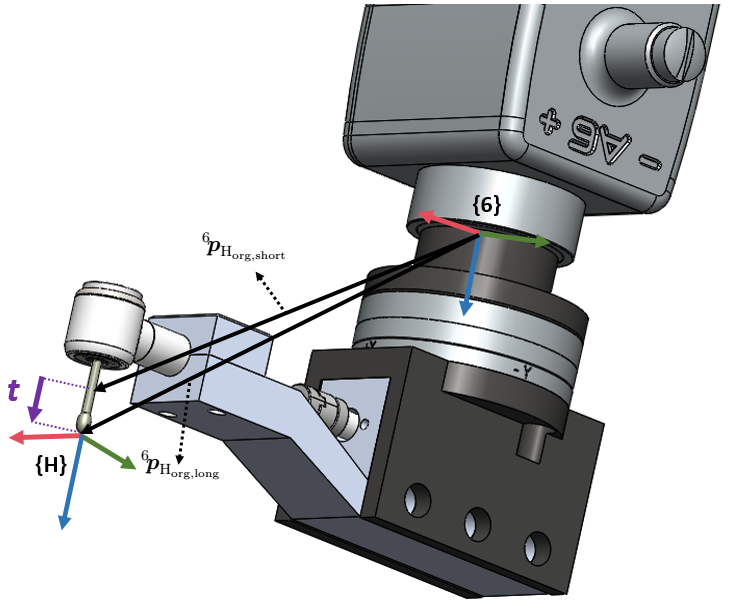
\includegraphics[width=0.7\linewidth]{Images/TCP2.png}
\caption{ 
Schematic diagram for obtaining the tool vector. 
}\label{fig:tcp2}
\end{center}
\end{figure}
\hspace*{6mm}We are turning now to the discussion about the rotation vector. Above all, we have to find the vector of tool insertion direction $\boldsymbol{t}$. We can obtain the translation vector from the origin of frame\{6\} to the tooltip through the TCP method. Accordingly, we use two root canal files with different lengths and apply the TCP method to separately obtain two vectors illustrated as Fig \ref{fig:tcp2}. Hence, 
\begin{equation}
\begin{split}
\boldsymbol{t} =\ ^\mathrm{6}\!\boldsymbol{p}_\mathrm{H_{org,long}} -\ ^\mathrm{6}\!\boldsymbol{p}_\mathrm{H_{org,short}}
\end{split}
\end{equation}
\begin{figure}[H]
\begin{center}
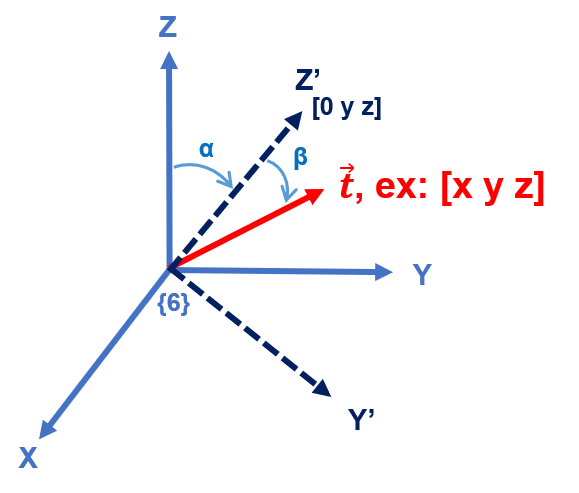
\includegraphics[width=0.6\linewidth]{Images/rot_inf.png}
\caption{
Illustration of finding the rotation matrix
}\label{fig:rot_inf}
\end{center}
\end{figure} 
For analyzing it easily, we depict it in Fig \ref{fig:rot_inf}. Note that here we only discuss rotation, so we assume that we have done translation and matched the frame\{S\} with frame\{6\}. Because we hope to send a Z-axis command to achieve tool insertion, we should align the original Z-axis to the target vector. Nevertheless, Z-axis alignment without other restrictions will produce many solutions. We choose one of the solutions to align Z-axis to the target vector. According to the figure, we assume the target vector $\boldsymbol{t}$ is $\left[x,y,z\right]$, whose projection to yz-plane $\mathrm{proj_{(y-z)}}\boldsymbol{t}$ is $\left[0,y,z\right]$. Initially, we rotate $\alpha$ degree around X-axis to make original Z-axis align the projection $\left[0,y,z\right]$. Next, we rotate $\beta$ degree around Y' axis and finally align the original Z-axis to the target vector [1,1,1]. The following equation 
\begin{equation}
\begin{split}
\ \  _{\mathrm{6}}^{\mathrm{T}}\mathbf{R} = \mathbf{R_x(\alpha)} \cdot \mathbf{R_y(\beta)}
\end{split}
\end{equation}
where
\begin{equation}
\begin{split}
\alpha &= 
-\mathrm{sign}(t_y)\cdot \cos^{-1} \left(  \frac{\hat{k}						\cdot 		\mathrm{proj_{(y-z)}}\boldsymbol{t}				}
								 				{\left \| \hat{k} \right \| 	\cdot \left \| \mathrm{proj_{(y-z)}}\boldsymbol{t} \right \|} \right)\ \\
\beta  &= 
\mathrm{sign}(t_x)\cdot \cos^{-1} \left( \frac{\textbf{t}							\cdot 		\mathrm{proj_{(y-z)}}\boldsymbol{t}			}
								  			  {\left \| \textbf{t}\right \| 	\cdot \left \| \mathrm{proj_{(y-z)}}\boldsymbol{t} \right \|} \right)\ 
\end{split}
\end{equation}
Assume $\boldsymbol{t} = [x,y,z]$,
\begin{equation}
\begin{split}
\alpha &= 
-\mathrm{sign}(y)\cdot \cos^{-1}	\left( \frac{z^2}{\sqrt{y^2+z^2}} \right) \mathrm{rad}\\
\beta  &= 
\mathrm{sign}(x)\cdot \cos^{-1} \left( \frac{y^2+z^2}{\sqrt{x^2+y^2+z^2}\sqrt{x^2+y^2+z^2}} \right) \mathrm{rad}
\end{split}
\end{equation}
$\alpha$ and $\beta$ are Euler angles, which meet the command demand.
\par
In this section, we have demonstrated two key aspects of reference frame changing of the robot arm. It's easy to input the results of section \ref{sec:tcp} and section \ref{sec:rot inf} via the command setTRF, the robot arm can recognize frame\{T\} and translate and orientate along with frame\{T\}. Having discussed how to combine a robot arm with an end effector, the next section addresses ways of combining an F/T sensor.